\documentclass{beamer}
%\usepackage[margin=1in]{geometry}
\usepackage{amsthm,amsmath,amsfonts,hyperref,graphicx,color,multicol}
\usepackage{enumitem,tikz}

%%%%%%%%%%
%Beamer Template Customization
%%%%%%%%%%
\setbeamertemplate{navigation symbols}{}
\setbeamertemplate{theorems}[ams style]
\setbeamertemplate{blocks}[rounded]

\definecolor{Blu}{RGB}{43,62,133} % UWEC Blue
\setbeamercolor{structure}{fg=Blu} % Titles

%Unnumbered footnotes:
\newcommand{\blfootnote}[1]{%
	\begingroup
	\renewcommand\thefootnote{}\footnote{#1}%
	\addtocounter{footnote}{-1}%
	\endgroup
}


%%%%%%%%%%
%Custom Commands
%%%%%%%%%%
\newcommand{\R}{\mathbf{R}}
\newcommand{\veca}{\vec{a}}
\newcommand{\vecb}{\vec{b}}
\newcommand{\vece}{\vec{e}}
\newcommand{\vecu}{\vec{u}}
\newcommand{\vecv}{\vec{v}}
\newcommand{\vecw}{\vec{w}}
\newcommand{\vecx}{\vec{x}}
\newcommand{\zerovector}{\vec{0}}

\newcommand{\ds}{\displaystyle}

\newcommand{\fn}{\insertframenumber}

\newcommand{\rank}{\operatorname{rank}}
\newcommand{\adj}{\operatorname{adj}}

\newcommand{\blank}[1]{\underline{\hspace*{#1}}}


%%%%%%%%%%
%Custom Theorem Environments
%%%%%%%%%%
\theoremstyle{definition}
\newtheorem{exercise}{Exercise}
\newtheorem{question}[exercise]{Question}
\newtheorem*{defn}{Definition}
\newtheorem*{exa}{Example}
\newtheorem*{disc}{Group Discussion}
\newtheorem*{nb}{Note}
\newtheorem*{recall}{Recall}
\renewcommand{\emph}[1]{{\color{blue}\texttt{#1}}}

\definecolor{Gold}{RGB}{237, 172, 26}
%Statement block
\newenvironment{statementblock}[1]{%
	\setbeamercolor{block body}{bg=Gold!20}
	\setbeamercolor{block title}{bg=Gold}
	\begin{block}{\textbf{#1.}}}{\end{block}}





\begin{document}
	\title{Math 324: Linear Algebra}
	\subtitle{Section 4.3:Subspaces of Vector Spaces}
	\author{Mckenzie West}
	\date{Last Updated: \today}
\begin{frame}
\maketitle
\end{frame}

\begin{frame}{\insertframenumber}
	\begin{block}{\textbf{Last Time.}}
	\begin{itemize}[label=--]
		\item Properties of $\vec 0$
		\item Abstract Vector Spaces
		\item Important Vector Spaces
	\end{itemize}
	\end{block}
	\begin{block}{\textbf{Today.}}
		\begin{itemize}[label=--]
			\item Proving Something is not a Vector Space
			\item Definition of Subspaces
			\item Test for Subspaces
		\end{itemize}
	\end{block}
\end{frame}
\begin{frame}{\fn}
\begin{statementblock}{Theorem 4.4}
	Let $\vec v$ be any element of a vector space $V$, and let $c$ be a scalar.  Then the following properties are true.
	\begin{enumerate}[label=\textbf{\arabic*.}]
		\item $0\vec v=\vec 0$
		\item $c\vec 0=\vec 0$
		\item If $c\vec v=\vec 0$, then $c=0$ or $\vec v=\vec 0$.
		\item $(-1)\vec v=-\vec v$
	\end{enumerate}
\end{statementblock}
\begin{exercise}
	Prove Theorem 4.4 property 1 following the steps on Canvas.
\end{exercise}
\end{frame}
\begin{frame}{\fn}
\begin{exercise}
	Verify all four of these results for the goofy vector space from last class: (first remind yourself of what $\zerovector$ and $-\vecv$ were)
	\begin{quote}
		$V=\{(x,y)\ :\ x,y\in\R \text{ and }y> 0\}$ with the operations:
		$$\begin{array}{rcl}	
		\text{Addition: \hspace*{.35in}} (x_1,y_1)\oplus (x_2,y_2)&=&(x_1+x_2,y_1y_2)\\
		\text{Scalar Multiplication: \hspace*{.1in}} c*(x,y)&=&(cx,y^c)
		\end{array}$$
	\end{quote}
\end{exercise}
\end{frame}

\begin{frame}{\fn}
	\begin{block}{\textbf{Brain Break.}}
		Would you rather fight 1 horse-sized duck or 100 duck-sized horses?
		\begin{center}
			
\includegraphics[width=2in]{../images/turducken_Pepper}
		\end{center}
	\end{block}
\end{frame}
%\begin{frame}{\fn}
%	\begin{exa}
%		To show that something is not a vector space, we simply have to give an example where one of the vector space axioms fails.  For example the collection $S$ of all continuous functions $f(x)$ such that $f(0)=1$ is not a vector space because:
%		
%			\begin{center}
%				\begin{minipage}{.8\textwidth}
%					If $f(x)=1$ then $(2f)(0)=2(f(0))=2(1)=2\neq1$, so $2f\not\in S $. Thus $S$ is not closed under scaling.\hfill\qedsymbol
%				\end{minipage}
%			\end{center} 
%	\end{exa}
%	\begin{exercise}
%		What other properties does the set from the previous example fail?
%	\end{exercise}
%\end{frame}
%\begin{frame}{\fn}
%	\begin{recall}
%		We can show something is not a vector space by showing that is fails a single one of the axioms. Here's some more practice with that.
%	\end{recall}
%	\begin{exercise}
%		Show that $\mathbb{Z}=\{\dots,-2,-1,0,1,2,3,\dots\}$ with the standard operations is not a vector space.
%	\end{exercise}
%	\begin{exercise}
%		Which of the 10 axioms fail for the set with $V=\R^2$ where we have the standard definition of addition but scalar multiplication is defined via:\[c(x,y)=(0,cy).\]
%	\end{exercise}
%\end{frame}
\begin{frame}{\fn}
	\begin{defn}
		A nonempty subset $W$ of a vector space $V$ is called a \emph{subspace} of $V$ when $W$ is a vector space under the operations of addition and scalar multiplication defined in $V$.
	\end{defn}
	\begin{exa}\begin{enumerate}[label=(\alph*)]
			\item $W=\{(x,x)\ :\ x\in \R\}$ is a subspace of $V=\R^2$
			\item $W=P_1$ is a subspace of $V=P_2$ (polynomials)
		\end{enumerate}
	\end{exa}
	\begin{block}{\textbf{Warning.}}
		$W=\R^2$ is NOT a subspace of $V=\R^3$ because elements of $\R^2$ are ordered pairs while elements of $\R^3$ are ordered triples.
	\end{block}
\end{frame}
\begin{frame}{\fn}
	\begin{nb}
	One nice thing about subspaces is that they use the same operations as something that is a vector space.  Therefore, axioms 2, 3, 7, 8, 9, and 10 are already known.
	\end{nb}
	\begin{statementblock}{Theorem 4.5 - Subspace Test}
		A subset $W$ of a vector space $V$ is a subspace if and only if the following hold.
		\begin{enumerate}[label=\textbf{\arabic*.}]
			\item $\vec0 \in W$ (or $W$ is non-empty).
			\item If $\vec u,\vec v\in W$, then $\vec u+\vec v\in W$.
			\item If $\vec u\in W$ and $c$ is a scalar then $c\vec u\in W$.
		\end{enumerate}
	\end{statementblock}
\end{frame}

\begin{frame}{\fn}
	\begin{exa}
		Proofs using Theorem 4.5 should use the following format.  Note: this is an essential type of proof to know.\\
		Claim: The set $\{(x,2x)\ :\ x\in\R\}$ with the standard operations on $\R^2$ is a vector space. 
		\begin{block}{Proof.}
			Let $W=\{(x,2x)\ :\ x\in\R\}$ with the standard operations on $\R^2$. We use The Subspace Test (Theorem 4.5).
			\begin{enumerate}[label=\textbf{\arabic*.}]
				\item Notice that $\vec0 =(0,0)$ is in $W$ as it is of the form $(x,2x)$ with $x=0$.
				\item Let $\vec u,\vec v\in W$.  Write $\vec u=(x,2x)$ and $\vec v=(y,2y)$ for $x,y\in\R$.  Then $\vec u+\vec v=(x,2x)+(y,2y)=(x+y,2x+2y)=(x+y,2(x+y))$, which is in the form of $W$.
			\end{enumerate}
		\end{block}
	\end{exa}
	(Continued on the next slide.)
\end{frame}
\begin{frame}{\fn}
	\begin{exa}[Cont.]
		\begin{block}{}
			\begin{enumerate}[label=\textbf{\arabic*.}]
				\item[\textbf{3.}] Let $c$ be a scalar. Then $c\vec u=c(x,2x)=(cx,c(2x))=(cx,2(cx))$, which is in the form of $W$.
			\end{enumerate}
			Therefore $W$ satisfies the subspace test and is a subspace of $\R^2$, so it is a vector space.\hfill$\square$
		\end{block}
	\end{exa}
\end{frame}

\begin{frame}{\fn}
	\begin{exercise}\label{subspaces}
		Use the subspace test to determine which of the following are vector spaces. For those that are, write a formal proof as in the example. For those that are not, give an example to explain why they are not.
	\begin{enumerate}[label=(\alph*)]
		\item The set $\{(x,0)\ :\ x\in\R\}$ with the standard operations on $\R^2$.
		\item The set $\{(a,-a,a+2)\ :\ a\in\R\}$ with the standard operations on $\R^3$.
		\item The set $D_n$ of $n\times n$ diagonal matrices with the standard operations on $M_n$.
		\item The set of $2\times 2$ matrices satisfying $A^2=A$ with the standard operations on $M_n$.
		\item The set of $2\times 2$ matrices of the form $\begin{bmatrix}0&b\\c&0\end{bmatrix}$ with the standard operations on $M_2$.
	\end{enumerate}
	\end{exercise}
\end{frame}

\begin{frame}{\fn}
\begin{block}{\textbf{Exercise \ref{subspaces} (Cont.)}}
	Use the subspace test to determine which of the following are vector spaces. For those that are, write a formal proof as in the example. For those that are not, give an example to explain why they are not.
	\begin{enumerate}[label=(\alph*)]\setcounter{enumi}{5}
		%\item The set of degree exactly 2 polynomials with the standard operations.
		\item The set $W=\{ax^2\ :\ a\in\R\}$ with the standard polynomial operations.
		\item The set of all even continuous functions.  Recall that a function is even if $f(-x)=f(x)$.
	\end{enumerate}
\end{block}
\end{frame}
%\begin{frame}{\fn}
%	\begin{exercise}
%		Solve the homogeneous system of equations with coefficient matrix \[A=\begin{bmatrix}1&1&1\\2&2&2\\3&3&3\end{bmatrix}.\]
%	
%	Is the set of solutions to this system a vector space with standard operations from $\R^3$?
%	\end{exercise}
%	\begin{exercise}
%		Let $A=\begin{bmatrix}1&2\\3&6\end{bmatrix}$ and $\vec b=\begin{bmatrix}-1\\-3\end{bmatrix}$.  Is the set of solutions to the system $A\vec x=\vec b$ a vector space with the standard operations in $\R^2$?
%	\end{exercise}
%\end{frame}
%\begin{frame}{\fn}
%	\begin{exercise}
%		Let $A$ be any $2\times 2$ matrix.  Prove that the set of solutions to the homogeneous system $A\vec x=\vec 0$ is a vector space by showing that it is a subspace of $\R^2$.
%	\end{exercise}
%\end{frame}
%\begin{frame}{\fn}
%	\begin{defn}
%		The \emph{intersection} of two sets is the set consisting of everything that appears in both sets, the shaded region in the Venn diagram below.  The intersection of $V$ and $W$ is denoted $V\cap W=\{\vec x\ :\ \vec x\in V \text{ and }\vec x\in W\}$.
%		\begin{center}
%			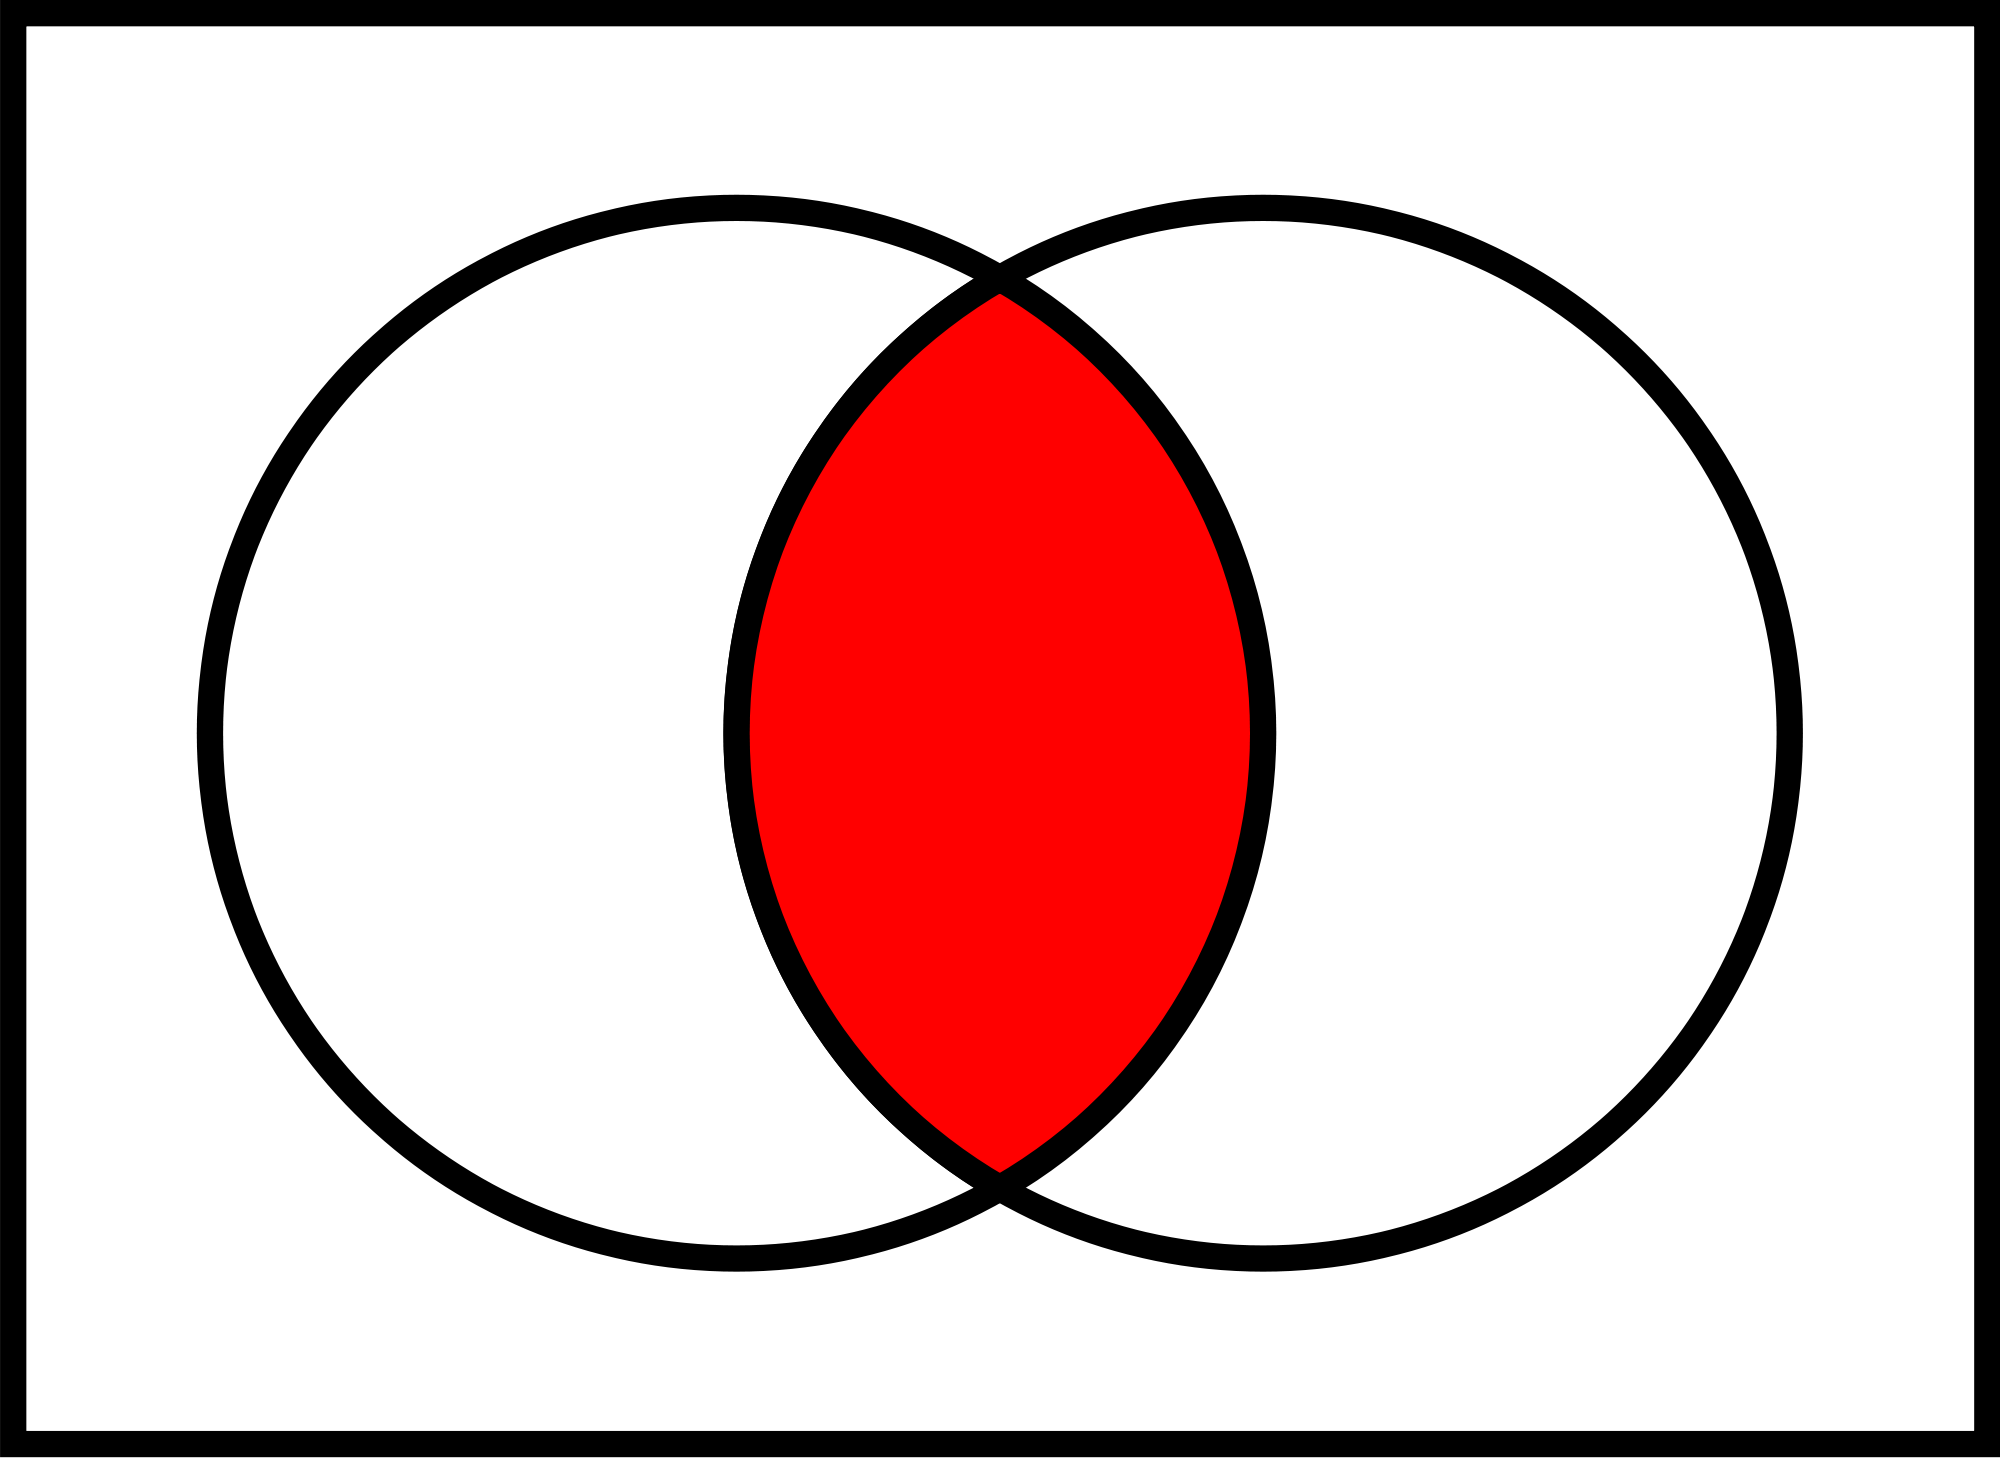
\includegraphics[width=1.5in]{../images/intersection}
%		\end{center}
%	\end{defn}
%	\begin{statementblock}{Theorem 4.9}
%		If $V$ and $W$ are both subspaces of a vector space $U$, then the {intersection} of $V$ and $W$ is also a subspace of $U$.
%	\end{statementblock}
%\end{frame}
%\begin{frame}{\fn}
%	\begin{exercise}
%		Complete the proof of Theorem 4.9.
%		\begin{proof}
%			Let $V$ and $W$ be subspaces of a vector space $U$.  We want to show that $V\cap W$ is a subspace of $U$ using the subspace test.
%			\begin{enumerate}[label=(\alph*)]
%				\item Explain why $\vec 0\in V\cap W$.
%				\item Let $\vec v$ and $\vec w$ be in $V\cap W$ this means that $\vec v$ and $\vec w$ are in $V$ and that $\vec v$ and $\vec w$ are in $W$.  Explain why $\vec v+\vec w$ is in $V\cap W$.
%				\item Let $\vec v$ be in $V\cap W$ and $c$ be a scalar.  Explain why $c\vec v\in V\cap W$ too.
%			\end{enumerate}
%		\end{proof}
%	\end{exercise}
%\end{frame}
%\begin{frame}{\fn}
%	\begin{exercise}
%		\begin{enumerate}[label=(\alph*)]
%			\item Prove that the set of points in $\R^3$ on the plane $x=0$ is a subspace of $\R^3$.  
%	
%			\item Prove that the set of points in $\R^3$ on the plane $y=0$ is a subspace of $\R^3$.
%	
%			\item Find the intersection of these planes and verify that it is also a subspace of $\R^3$. 
%		\end{enumerate}
%	\end{exercise}
%\end{frame}
%\begin{frame}{\fn}
%	Just like in the case of $\R^n$ we can consider linear combinations for general vector spaces.
%	\begin{defn}
%		A vector $\vec v$ in a vector space $V$ is a \emph{linear combination} of $\vec u_1,\vec u_2,\dots,\vec u_n\in V$ if there exist scalars $c_1,c_2,\dots,c_n$ such that
%			\[\vec v=c_1\vec u_1+c_2\vec u_2+\cdots+c_n\vec u_n.\]
%	\end{defn}
%	\begin{exa}
%		The polynomial $p(x)=3+x-2x^2$ is a linear combination of $q_1(x)=1+x$, $q_2(x)=1+x^2$, $q_3(x)=1+x+x^2$, and $q_4(x)=x^2$ because \begin{eqnarray*}p(x)&=&3+x-2x^2\\ &=&5(1+x)+2(1+x^2)-4(1+x+x^2)+0x^2\\&=&5q_1(x)+2q_2(x)+(-4)q_3(x)+0q_4(x)\end{eqnarray*}
%	\end{exa}
%\end{frame}
%\begin{frame}{\fn}
%	\begin{exercise}
%			Can the polynomial $p(x)=1-4x+x^2$ be written as a linear combination of $q_1(x)=1+x$ and $q_2(x)=1+x^2$?
%	\end{exercise}
%	\begin{exercise}
%		Describe all of the polynomials can be written as a linear combination of $q_1(x)=1+x$ and $q_2(x)=1+x^2$.
%	\end{exercise}
%\end{frame}
\end{document}

